\documentclass[9pt,journal,a4]{IEEEtran}

\usepackage{cite}
\usepackage{amsmath}
\usepackage{graphicx}
\usepackage{textcomp}
\usepackage{booktabs}
\usepackage{stfloats}
\graphicspath{{figures/}}

\begin{document}

\title{From Individual Uncertainty to Collective Predictability: Consumer Aggregation and the Identifiability of Thermostatic Loads}

\author{Alexandre~M.~V.~Gouveia}

\maketitle

\begin{abstract}
Electric Thermostatic Loads (ETLs) impose temperature-correlated demand on low-voltage (LV) networks, yet a Distribution System Operator (DSO) sees only aggregated net load and rarely the number of consumers behind it. This paper treats the level of consumer aggregation as the variable that governs what a temperature-response fit to net load can reveal. Aggregation acts in two opposing directions: it renders the fit predictable, since idiosyncratic demand averages out while the temperature-driven component does not, and it renders the fit ambiguous, since the response of ordinary consumers accumulates alongside that of the ETLs. On smart-meter data from three countries, fit quality is shown to rise monotonically with the consumer count and to reproduce unchanged on two unseen datasets, one driven by cooling rather than heating. The difficulty of reading an ETL from the fit is then shown to be an unknown consumer count rather than a large one: at a known count, ETL-bearing substations separate from ETL-free ones essentially perfectly, and normalisation recovers most of what not knowing the count costs. Aggregation is found to buy precision rather than correctness, with the same transition sharpening the fitted simultaneity factor of the ETL population.
\end{abstract}

\begin{IEEEkeywords}
Electric thermostatic loads, heat pumps, low-voltage networks, degree-day regression, smart meter data, distribution system observability.
\end{IEEEkeywords}


\section{Introduction}
\label{section:intro}

Electrification of heating and cooling, driven by decarbonisation policy, is placing Electric Thermostatic Loads (ETLs) on low-voltage (LV) networks that were not sized for them~\cite{Lov17, Bec24}. Their demand is strongly correlated with ambient temperature~\cite{Che21b}, so its aggregate behaviour is in principle visible in the net load a Distribution System Operator (DSO) already meters. What the DSO generally lacks is the context needed to interpret that behaviour: appliance registers, nameplate ratings and, critically, the number of consumers a substation serves~\cite{Gou26}.

Previous work establishes the load--temperature relationship either from submetered thermal load, where the thermal contribution is directly observable~\cite{Fei13, Wei20b, Bru23}, or at a single fixed level of aggregation using change-point and degree-day regression~\cite{Ruc92, Per17b}. The aggregation level itself has not been treated as the variable that governs what remains identifiable, even where net-load disaggregation is performed at the substation~\cite{Wan20}. Yet it is not a fixed property of the problem: it varies between substations, is generally unknown to the DSO, and governs both how clearly the thermal response appears and how ambiguous its origin is.

This paper makes three contributions. It formalises consumer aggregation as the governing variable in the identifiability of ETLs from aggregated LV net load, separating the predictability that aggregation confers from the attributability it removes. It implements two use cases derived from a single fit, namely Detection and Energy Estimation, and reports each against the aggregation level. It reproduces the aggregation effect on two previously unseen datasets from different climates and building stocks, one driven by cooling rather than heating, without recalibrating the fitting procedure.


\section{Aggregation and Identifiability}
\label{section:identify}

\subsection{Thermal Response and its Two Aggregation Effects}

At the individual level an ETL is thermostatically controlled and strongly intermittent: a single device is either running or idle, and its instantaneous demand is a poor indicator of the temperature that caused it. Aggregation over the consumers downstream of an LV substation removes that intermittency, as thermostatic cycling decorrelates between dwellings and idiosyncratic occupancy averages out. The aggregate net load is then smooth and approximately piecewise linear in temperature, a form long used in change-point and energy-signature analysis of building and community load~\cite{Ruc92, Ali11, Per17b},
\begin{equation}
P(T) = P_{\mathrm{base}} + s_h \max\left(0,T_h-T\right) + s_c \max\left(0,T-T_c\right),
\label{eq:thermal-response}
\end{equation}
where $P_{\mathrm{base}}$ is the temperature-independent load [kW], $s_h$ and $s_c$ are the heating and cooling Thermal Sensitivities [kW/$^\circ$C], and $T_h \leq T_c$ bound a dead band over which no thermal response is present. Fitting is performed on daily aggregates, which averages out occupancy-driven variability and building thermal inertia that are not temperature-dependent. The model is thus a description of a population rather than of a consumer, and the population size is a condition for it to hold at all.

The first effect of increasing the consumer count $N$ is to improve how well Equation~\eqref{eq:thermal-response} describes the data, since averaging over more consumers suppresses the idiosyncratic component while leaving the temperature-driven one intact. The second effect runs the other way. Consumers without an ETL are not thermally inert, as lighting and occupancy correlate with the seasonal cycle, so the heating sensitivity decomposes as
\begin{equation}
s_h = N \sigma_{\mathrm{base}} + N_{\mathrm{etl}} \sigma_{\mathrm{etl}},
\label{eq:sensitivity-decomposition}
\end{equation}
where $N_{\mathrm{etl}}$ is the ETL count, $\sigma_{\mathrm{base}}$ the mean per-consumer non-thermal sensitivity and $\sigma_{\mathrm{etl}}$ the mean per-load thermal sensitivity. The residual per-consumer term is more than an order of magnitude smaller than the per-load term, yet it accumulates with substation size. A given $s_h$ is therefore consistent with many $(N, N_{\mathrm{etl}})$ pairs, so aggregation buys a better-determined curve at the cost of a more ambiguous one.

The obstruction is not identification at a large $N$ but at an unknown $N$: were the consumer count published, the reference contribution $N \sigma_{\mathrm{base}}$ could be subtracted and the ambiguity would not arise. Where $N$ is unknown, normalising $s_h$ by an observable that scales with it, such as the substation peak load, removes most of the dependence, and this route is adopted below.

\subsection{Identifiable Quantities}

Two use cases follow from Equation~\eqref{eq:thermal-response}, differing in how much of the aggregation level each needs to be known. \textbf{Detection} assesses ETL presence by comparing a normalised sensitivity against a reference distribution from substations known to contain none, a task usually posed at the individual meter~\cite{Fei13, Wei20b}. \textbf{Energy Estimation} integrates the thermal term over a day's temperature to recover the temperature-driven energy consumed, the aggregate analogue of heat-pump load disaggregation~\cite{Bru23}. Neither yields the installed capacity of the ETLs, which requires the ratio between aggregated demand and summed rated powers that net load does not identify.


\section{Aggregation Makes the Fit Predictable}
\label{section:predictable}

The use cases are implemented on the HEAPO dataset~\cite{Bru25} complemented with Swiss smart-meter data providing submetered thermal load, giving net load at 15-minute resolution for 1702 LV consumers over 2023, of which 81 carry a submetered heat pump. Heat pumps are the only ETL with a submetered thermal series, so they are the ETL used throughout. Synthetic substations are drawn from this pool over a factorial grid of consumer count $N$ and ETL count $N_{\mathrm{etl}}$, at 25 replicates per cell. Because only 81 submetered heat pumps supply the ETL tier, intervals below are obtained by resampling consumers rather than substations, so the spread reflects the consumer population rather than the draw.

Fig.~\ref{fig:aggregation} reports median net-load $R^2$ against the averaging window, one line per consumer count, at a fixed 50\% penetration. Fit quality rises with $N$ at every window, from 0.71 at $N=4$ to 0.92 at $N=48$ at 25\% penetration, and the gain is largest where the ETL signal is weakest. The reference group shows the effect in isolation: substations carrying no ETL reach a median $R^2$ of 0.19 at $N=4$ against 0.52 at $N=48$, so aggregation renders identifiable a temperature response that no ETL produces. The fitted parameters stabilise alongside the fit, the relative spread of $s_h$ across replicates falling from 0.37 to 0.22 over the same range.

\begin{figure*}[t]
\centering
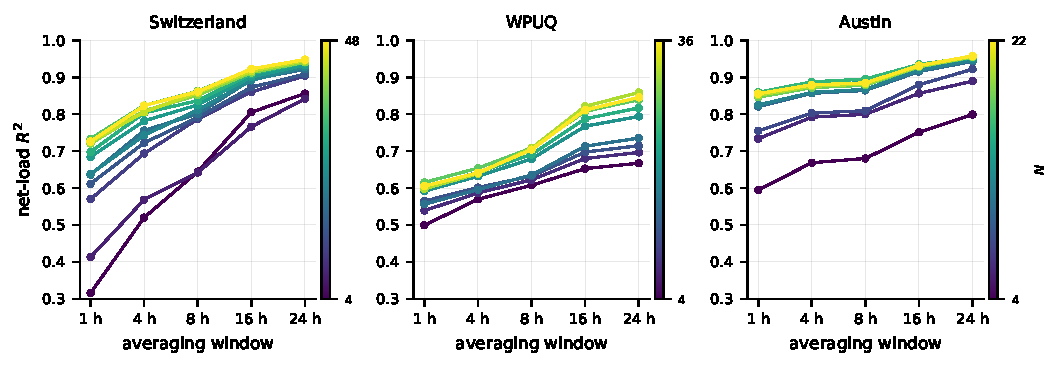
\includegraphics[width=0.92\textwidth]{figures/fig_aggregation_three.pdf}
\caption{Median net-load $R^2$ against averaging window, one line per consumer count, for the three datasets. Switzerland is the factorial training design at 50\% penetration; WPUQ and Austin are nested sequences in which each aggregate contains the one below it. Fit quality rises with the consumer count on all three, and the direction is preserved though the levels differ.}
\label{fig:aggregation}
\end{figure*}

The effect reproduces on two unseen datasets (Fig.~\ref{fig:aggregation}). WPUQ is 37 German single-family houses on one LV feeder for 2019, each with a separately metered heat pump~\cite{Sch22}; net-load $R^2$ at 24~h rises from 0.67 to 0.85 over a nested sequence adding consumers to a fixed aggregate. Pecan Street's Austin panel is 22 air-conditioned dwellings for 2018~\cite{pecanstreet}, driven by cooling rather than heating, with both arms of Equation~\eqref{eq:thermal-response} free; there $R^2$ rises from 0.80 to 0.96. The levels are lower, yet the direction holds across a change of country, climate, building stock and thermostatic technology, so it follows from aggregation itself rather than from any one dataset.


\section{What Aggregation Makes Identifiable}
\label{section:identifiable}

\subsection{Detection}

A least-squares fit of Equation~\eqref{eq:sensitivity-decomposition} across the median sensitivity surface gives $\sigma_{\mathrm{etl}}=0.117$ against $\sigma_{\mathrm{base}}=0.0054$~kW/$^\circ$C, so a single ETL is worth about 22 ordinary consumers of raw sensitivity. The size dependence is severe enough to invert a ranking: a 48-consumer substation with no ETL out-slopes a 4-consumer one at 50\% penetration. Pooled over substations of different and unknown size, the raw sensitivity separates ETL-bearing from ETL-free substations at an Area Under the Curve (AUC) of 0.974, and peak normalisation raises this to 0.990, comparable to meter-level detectors trained on labelled data~\cite{Wei20b, Fei13}.

These pooled figures understate what the fit recovers. Computing the AUC within each consumer count separately, so that positives and negatives share a known $N$, gives a median of 1.000 for the raw sensitivity, reaching exactly unity at 8 of the 12 sizes and never below 0.990 (Fig.~\ref{fig:within-stratum}). Separation is therefore essentially perfect at every aggregation level, including the smallest. The difficulty Detection faces is an unknown $N$, not a large one. The gap between the two views measures that difficulty: 0.026 for the raw sensitivity, which peak normalisation reduces to 0.006. The ranking inverts, the raw sensitivity being the best discriminator at known $N$ and the worst at unknown $N$, since normalising by a noisy observable costs accuracy where no size correction is needed.

\begin{figure}[t]
\centering
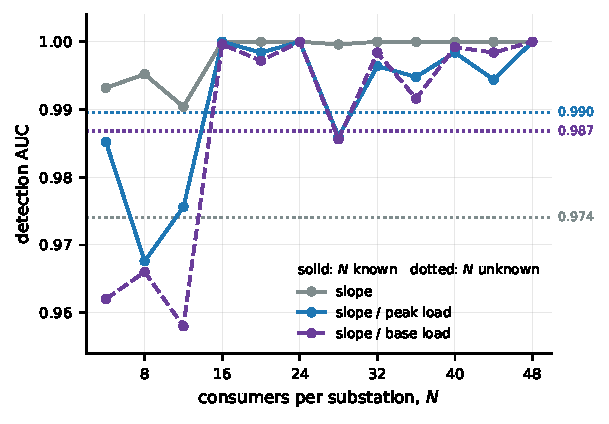
\includegraphics[width=0.9\columnwidth]{figures/fig_within_stratum_auc.pdf}
\caption{Detection AUC against consumer count, scored within each count so that positives and negatives share a known $N$ (solid), against the same statistic pooled over every $N$ (dotted). The vertical gap is the cost of not knowing $N$, and the ranking of the three statistics inverts between the two views.}
\label{fig:within-stratum}
\end{figure}

A 95\% specificity is nonetheless a weak guarantee where ETLs are sparse: at a deployment prevalence of 5\% the Positive Predictive Value is 0.50, so the statistic is better used to rank substations for inspection than to classify them outright.

\subsection{Energy Estimation and Coincidence}

Pooled across 438\,000 substation-days, the thermal term reaches $R^2=0.953$ against submetered thermal energy at a total-energy bias of $-11.5\%$, a quantity the fit never saw, since its target was net load. Accuracy again improves with the consumer count, most where penetration is lowest: at 25\% penetration the per-substation $R^2$ dispersion contracts from an interquartile range of 0.47 at $N=4$ to 0.08 at $N=48$, so aggregation buys reliability across substations more than accuracy at the typical one. The bias, by contrast, is invariant to $N$, holding near $-11\%$ throughout, since it follows from the dead band of Equation~\eqref{eq:thermal-response} rather than from the sample: ETL energy persisting above $T_h$, most plausibly domestic hot water, is unrepresented by construction.

The same individual-to-collective transition sharpens the Simultaneity Factor (SF) of the heat pump population, the fraction of connected load drawing power at once, a quantity central to how aggregate heat-pump demand and coincidence are characterised for network planning~\cite{Lov17, Che21b}. A single heat pump is either running or idle, so its coincident fraction is degenerate. Aggregation renders it a stable fraction: the median SF at the coldest observed day holds near 0.42, while its interquartile range across substations collapses from 0.162 at one heat pump to 0.007 at 48 (Fig.~\ref{fig:simultaneity}). Aggregation does not so much reveal a coincidence value as render a fixed one certain. The SF is reported to characterise the aggregation, not as an operating quantity, since it is built from the submetered load and installed peak a DSO does not hold, and its absolute level reflects local climate and sizing rather than a value that transfers.

\begin{figure}[t]
\centering
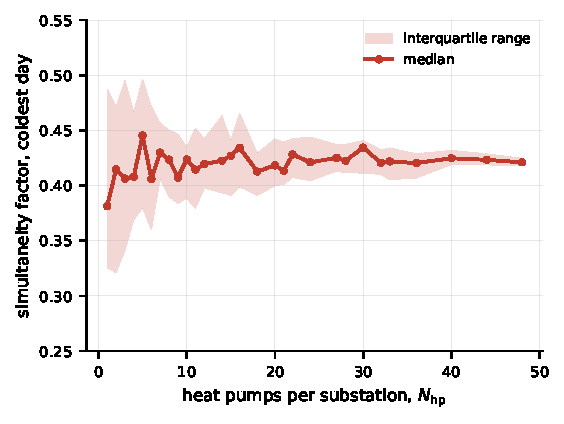
\includegraphics[width=0.9\columnwidth]{figures/fig_sf_by_aggregation.pdf}
\caption{Fitted simultaneity factor at each substation's coldest observed day, against the number of heat pumps aggregated. The median holds near 0.42 while the interquartile band funnels in, from 0.162 at a single heat pump to 0.007 at 48.}
\label{fig:simultaneity}
\end{figure}


\section{Discussion and Conclusion}
\label{section:discussion}

Aggregation is what renders these loads visible, and what renders them ambiguous. What it buys is precision rather than correctness: fit quality and Energy Estimation sharpen with the consumer count, most where the ETL signal is weakest, yet the systematic bias is invariant to aggregation. What it costs is attributability, as the reference term of Equation~\eqref{eq:sensitivity-decomposition} accumulates alongside the ETL term, leaving a well-fitted curve ambiguous about its origin until a known consumer count, or a normalisation, resolves it.

The behaviour transfers even where the values do not: fit quality rises with the consumer count on all three datasets, whereas the absolute Thermal Sensitivities reflect local building stock and climate and are not expected to. The use cases themselves rest on the training data alone, since WPUQ contains no genuinely ETL-free consumer against which to score Detection. Both require only net load and ambient temperature to run, the household survey serving to build and validate the design rather than to operate the method.

No single aggregation level is preferable across both use cases. Larger substations yield better-determined fits and more accurate energy estimates, whereas Detection is already saturated at the smallest size tested. Where a consumer count is available it is worth more than additional aggregation, and where it is not, the normalised statistic recovers most of what its absence costs. The latter is the condition under which a DSO actually operates, and publishing consumer counts alongside aggregated substation consumption would measurably improve what can be read from net load.


\bibliographystyle{IEEEtran}
\bibliography{references_letter}

\end{document}
